\documentclass{aas}
% Individual identity supplied by the author on 2026-11-09.
\newcommand{\AuthorName}{蒋佳豪}
\newcommand{\StudentID}{22671064}
\newcommand{\CourseName}{工程技术前沿}
\newcommand{\ReviewTitle}{面向科研任务的多智能体系统综述}
\newcommand{\ReviewSubtitle}{知识、记忆与协作的机制及证据边界}
\newcommand{\ReportDate}{2026年11月9日}

\usepackage{journal-review}
\begin{document}
\twocolumn[{
\articleheading
\begin{minipage}{\textwidth}\fontsize{10}{14.8}\selectfont
\abstractlabel{摘\quad 要}
大语言模型正推动科研辅助由文献问答和代码生成，向涵盖假设提出、实验执行及结果论证的连续工作流发展。
多智能体系统通过任务分解、角色协作和工具调用，为复杂研究过程提供了新的组织方式，
其研究重点也逐渐从单项任务性能转向长期协作能力与科学产出的有效性。
本文围绕知识增强、长期记忆、协作控制和可信评价，梳理科研多智能体系统的发展脉络与主要技术路线。
首先建立研究流程与支撑机制相结合的分类框架，比较片段检索、层次检索、图组织、反思记忆及多种协作拓扑；
继而分析文献综合、假设生成、计算实验和实体实验中的代表性系统，讨论其自动化范围、反馈来源与验证方式。
结合科学任务基准和过程审计的公开结果，进一步辨析执行成功与任务完成、候选排序与科学验证之间的差异。
在此基础上，本文认为知识结构与研究状态的协同维护、探索资源与验证资源的合理分配，
以及人工判断在关键研究节点的参与，是提高系统实用性的重要方向。
未来研究需要在可追溯证据、长期任务评价和可复现流程的基础上，检验多智能体协作带来的实际科研增益。
\par\vspace{2mm}
\abstractlabel{关键词}科研智能体；多智能体协作；检索增强生成；长期记忆；科学发现；可信评价
\par\vspace{3mm}
\begin{center}\fontsize{12}{16}\selectfont\bfseries
A Review of Multi-Agent Systems for Scientific Research:\\
Technical Evolution, Core Methods and Trustworthy Evaluation
\end{center}\vspace{1mm}
\abstractlabel{Abstract}
Large language models are extending research assistance from literature question answering and code generation to workflows that include hypothesis formulation, experimentation and scientific argumentation.
Multi-agent systems organize these capabilities through task decomposition, role coordination and tool use.
This review traces their development and synthesizes four technical dimensions: knowledge augmentation, long-term memory, collaborative control and trustworthy evaluation.
It compares retrieval structures, reflective memory and communication topologies, then examines representative systems for literature synthesis, hypothesis generation, computational research and physical experimentation.
Published benchmark and auditing results are used to distinguish executable programs from successful research tasks, and candidate ranking from empirical validation.
The discussion identifies coordinated knowledge and state management, balanced allocation of exploration and verification resources, and human participation at critical decisions as priorities for practical research systems.
Future progress requires evaluations grounded in traceable evidence, reproducible workflows and sustained research tasks.
\par\vspace{2mm}
\abstractlabel{Keywords}scientific agents; multi-agent collaboration; retrieval-augmented generation; long-term memory; scientific discovery; trustworthy evaluation
\end{minipage}\vspace{6mm}}]
\thispagestyle{plain}
% BODY-BEGIN
\section{引言}
一项研究从文献阅读推进到实验和结论，需要在多种信息与方法之间作出连续判断。
找到一篇相关论文之后，研究者还要判断其中的条件能否迁移到当前问题；完成一次计算之后，也要决定结果是否足以支持原先的解释。
这类工作既依赖专业知识，又涉及阅读、实现、比较和修正等连续活动。
大语言模型（large language model，LLM）能够在同一语言接口下调用检索、编程与分析工具，使上述活动有可能被纳入相对统一的自动化过程。
科研智能体研究正是在这一背景下兴起\cite{surveyautonomy,surveyagentic}。

检索增强生成（retrieval-augmented generation，RAG）使模型能够利用训练之外的文献\cite{rag}；
ReAct让模型依据工具返回的观察继续行动\cite{react}；AutoGen则提供了组织多个模型实例及其交互的方式\cite{autogen}。
这些方法解决的是不同层次的问题，却常被同时用于一个科研系统。
检索者、程序编写者、评审者等角色由此进入研究流程，形成了目前常见的科研多智能体架构。
本文中的“代理”与“智能体”同义；角色是否构成有效分工，取决于其信息和操作上的差异。

随着系统能够承担的研究步骤增多，完成流程仍不足以保证结论得到支持。
The AI Scientist能够组织实验并生成论文\cite{scientistjournal}，Virtual Lab将跨学科讨论落实到纳米抗体设计与实验表征\cite{virtual}，
对自动科研的审计却发现，最终报告有时不足以暴露实验过程中的方法学缺陷\cite{pitfalls}。
三类结果并不冲突：它们分别考察自动化覆盖、特定科学任务和过程可靠性。
如果只问系统是否“像科学家”，这些差异很容易被同一个概念掩盖。

已有综述对此给出了不同的整理方式。
Zheng等按工具、分析者和科学家区分自主程度\cite{surveyautonomy}；Wei等将系统能力与学科应用联系起来\cite{surveyagentic}；
郑逸宁等则细分了工具使用的规划、指令生成与结果处理\cite{surveytool}。
本文在这些工作的基础上，围绕三个相互关联的问题展开：系统怎样取得并保存研究依据，多个代理怎样据此协作，现有实验又怎样证明这种协作有用。
相比按框架逐项介绍，这一线索更便于解释方法之间的替代关系，也能把课堂涉及的知识图谱、自主记忆和可信科研放在同一个问题下讨论。

本文采用叙述性综述方法，通过题名与关键词检索、引用追踪以及原文核对选取代表工作，资料范围截至2026年11月9日。
分析包括基础机制、科研系统与评价研究，不覆盖全部多智能体强化学习或机器人群体研究，也不进行跨论文效应合并。
同一项目的不同版本按研究进展引用，例如The AI Scientist的早期报告、第二版与期刊稿不作为相互独立的重复验证。
下文先厘清研究对象，再讨论知识、记忆与协作方法；随后以科研应用和公开评测检验这些方法的解释力，最后给出本文的判断及尚未解决的问题。

\section{发展脉络与技术框架}
\subsection{从工具增强到研究流程组织}
科研智能体的发展并非单一路线的替代，而是知识获取、工具使用和过程组织逐步结合的结果，见图\ref{fig:timeline}。
RAG将非参数化检索与语言生成联系起来，使回答可以利用训练之外的资料\cite{rag}。
ReAct进一步通过行动获取环境观察，使检索和执行结果能够影响后续推理\cite{react}。
Toolformer则从训练角度研究模型如何决定调用何种工具、传入哪些参数以及怎样利用返回值\cite{toolformer}。
三者分别改变了信息来源、交互过程和工具调用能力，构成了科研助手进入外部环境的基础。

在此基础上，研究者开始处理长任务中的经历保留与角色协调。
Reflexion将任务反馈转化为可供后续尝试使用的文字反思\cite{reflexion}，
Generative Agents和MemGPT分别探索经历检索与分层存储\cite{generative,memgpt}。
AutoGen与MetaGPT则从代理交互、标准化交付和流程约束等角度组织多个模型实例\cite{autogen,metagpt}。
这些机制使研究活动不必在每次模型调用后重新开始，也使复杂任务可以被拆分为相互衔接的子任务。

面向科学研究的系统进一步把上述能力组合到具体场景。
ResearchAgent和SciAgents侧重利用文献关联生成研究方向，Agent Laboratory组织计算研究流程，
AI co-scientist强调候选假设的生成与演化，而Virtual Lab和Coscientist将规划与实体实验联系起来\cite{researchagent,sciagents,lab,cosci,virtual,chem}。
2026年的The AI Scientist期刊研究进一步同时讨论模板驱动和开放搜索两种模式\cite{scientistjournal}。
这些进展表明，研究焦点已由模型能否完成单个步骤，转向多个步骤如何组成可持续运行、可评价的研究过程。

\begin{figure*}[t]\centering
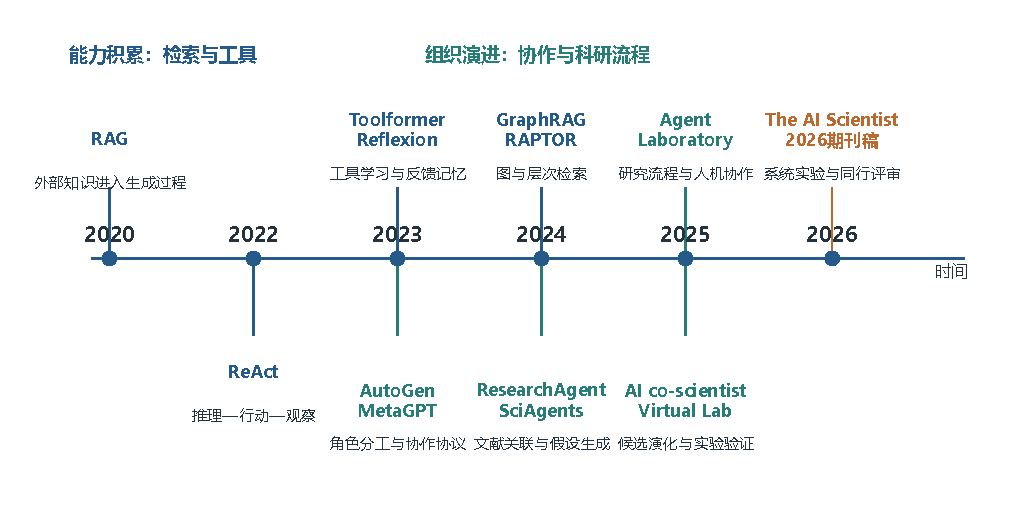
\includegraphics[width=\textwidth]{figures/review-timeline.pdf}
\caption{科研智能体相关能力与系统的代表性发展脉络。依据文献\cite{rag,react,toolformer,reflexion,autogen,metagpt,graphrag,raptor,researchagent,sciagents,lab,cosci,virtual,scientistjournal}整理。
基础工作按首次报告年份归类，2026年节点指期刊报告；时间节点为离散排布，不以间距表示持续时间。图中仅列代表工作，不表示其他路线在相应年份缺失。}
\label{fig:timeline}\end{figure*}

\subsection{科研工作流中的功能分层}
从工作流看，科研活动可以概括为问题形成、方案与实现、观察与分析、论证与交流四个相互联系的阶段。
实际研究往往在这些阶段之间往返，因而系统需要同时管理材料、状态和控制，见图\ref{fig:framework}。
知识获取负责提供外部论文、数据和工具说明；长期记忆保存项目经历及其解释；
协作控制负责选择动作、分配任务、整合输出并决定返工或停止。
三类机制分别对应信息可获得性、任务连续性与过程协调性。

这种分层有助于区分系统能力的来源。
模型没有找到相关结果，可能是检索覆盖不足；已经检索到的材料被后续阶段遗忘，涉及状态管理；
材料和状态均存在但任务仍然偏离目标，则需要检查计划与交接规则。
如果只用最终答案分数描述系统，这些性质不同的问题就容易被归入同一类“模型能力不足”。
功能分层并不要求物理上部署独立模块，而是为方法比较、系统消融和失败定位提供统一的描述方式。

\begin{figure*}[t]\centering
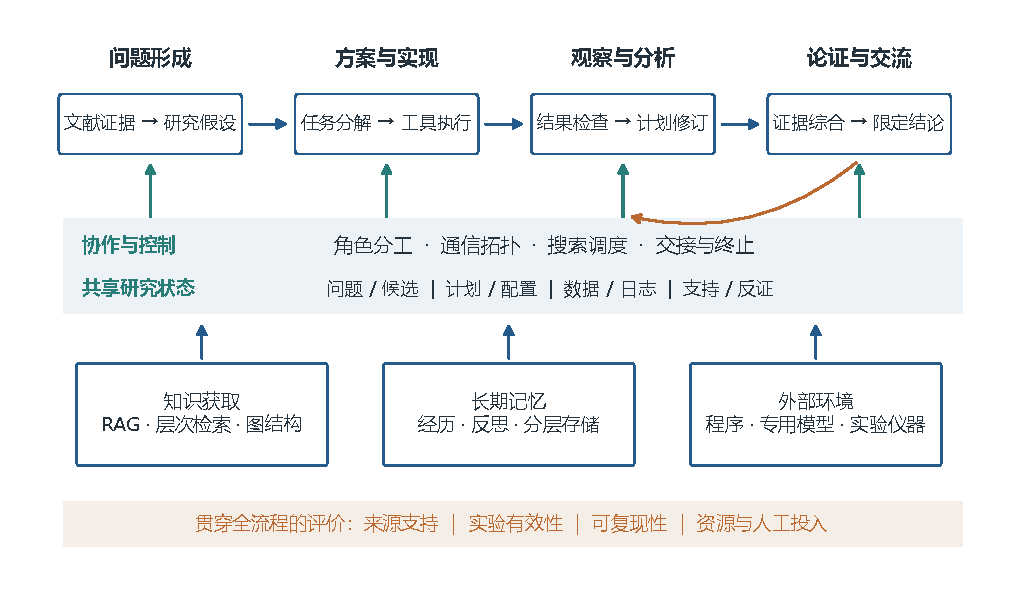
\includegraphics[width=\textwidth]{figures/review-framework.pdf}
\caption{科研工作流与支撑机制的对应关系。综合检索增强、分层记忆、代理交互与自动科研流程\cite{rag,memgpt,autogen,lab,scientistjournal}绘制。
上部为研究阶段，中部为协作及共享状态，下部为知识、记忆和环境支撑；评价贯穿整个过程。该图为综述性归纳，箭头不表示测得的效果大小。}
\label{fig:framework}\end{figure*}

\subsection{单智能体与多智能体的关系}
智能体通常由基础模型、可用工具、状态及动作选择规则共同构成。
在给定研究目标$g$下，其行为可抽象为
\begin{equation}
 a_t\sim\pi_\theta(a\mid g,o_{\leq t},m_t),
\end{equation}
其中$o_{\leq t}$为已有观察，$m_t$为当前记忆状态，$a_t$可以是检索、执行、通信或终止等动作。
该式仅用于统一描述，并不限定策略必须通过训练获得。
多智能体系统在此基础上引入不同主体之间的信息交换、任务依赖和调度规则。

因此，多智能体与单智能体之间并不存在只由数量决定的能力分界。
一个具有检索和执行反馈的代理可以完成较复杂的循环，多个代理也可能只是在重复相同推理。
多代理的实际价值取决于分解后的任务是否具有互补性、角色能否获得不同观察，以及协调开销是否小于分工收益。
本文在后续比较中将基础模型、工具能力、协作结构与计算预算分别处理，避免把系统层面的所有改进都归因于代理数量。

\section{知识增强与长期记忆}
\subsection{检索粒度与知识组织}
科研任务需要处理的资料既包括局部事实，也包括跨文献的主题、方法和争议。
不同查询所需的检索粒度并不相同：查找实验参数通常需要原文片段，比较多项研究则需要整合其对象、条件与结论。
RAG的原始研究将文档检索与条件生成结合，为利用外部知识提供了通用途径\cite{rag}。
其优势在于资料可以更新，生成结果也有机会回到明确来源；不足是局部相似性并不总能覆盖问题所需的全部信息。
当答案依赖多处条件时，单个高相似片段可能不足以支持完整判断。

层次检索通过改变信息的组织尺度缓解这一问题。
RAPTOR递归地对文本片段进行聚类和摘要，构建包含不同抽象层次的树，使检索同时接触细节与较高层概括\cite{raptor}。
与直接增加返回片段数量相比，这类方法能够显式表示信息的概括关系。
但摘要层次越高，压缩越明显，关键限定与原始证据之间的距离也越大。
因此，层次摘要适合定位主题和组织阅读，涉及具体数值或争议判断时仍需向下追索。

GraphRAG采用另一种组织方式：从文本中抽取实体及关系，通过社区发现和社区摘要形成全局信息结构\cite{graphrag}。
其主要价值是支持面向整个语料的概括，特别是相关信息分布在多个文档中的问题。
相较于树结构，图能够容纳更丰富的交叉关系，但也增加了实体消歧、关系抽取与更新维护的复杂度。
RAPTOR与GraphRAG因而分别强调层次概括和关系连接，并非彼此完全可替代的索引方案。
图\ref{fig:knowledge}从信息组织角度比较了这些路线与任务记忆的差别。

\begin{figure*}[t]\centering
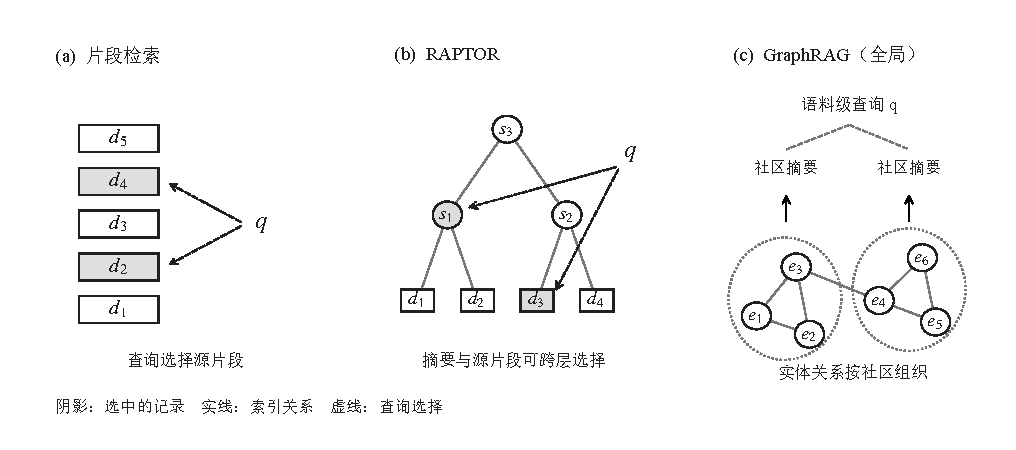
\includegraphics[width=\textwidth]{figures/review-knowledge-memory.pdf}
\caption{外部知识与研究记忆的组织方式。左、中两部分分别根据RAG、RAPTOR及GraphRAG的机制绘制\cite{rag,raptor,graphrag}；
右部综合MemGPT、Reflexion与科研状态管理需求\cite{memgpt,reflexion}，为本文分析示意，不代表原方法使用了完全相同的状态字段。各结构不按存储量或性能比例绘制。}
\label{fig:knowledge}\end{figure*}

\subsection{检索决策与证据支持}
除索引结构外，检索何时发生、结果如何被筛选，同样影响生成质量。
Self-RAG使用经过训练的反思标记，控制是否检索，并评价材料相关性、生成内容的支持程度及回答质量\cite{selfrag}。
与固定返回若干片段的流程相比，这一路线把检索需求和证据使用纳入生成决策。
它也说明“反思”可以具有不同技术含义：Self-RAG包含专门训练和控制标记，
并不是在任意模型之后添加一句检查提示就能获得相同机制。

面向科研的证据使用还需要区分相关、支持与充分三个层次。
某段文字可以与问题相关，却只讨论另一种数据设置；即使支持一个局部命题，也未必足以支持更广泛结论。
因此，检索输出需要保留对象、实验条件和结论范围，生成阶段则应维持这些限定。
在检索结果互相矛盾时，较合理的输出是呈现差异及其可能来源，而非强行综合成一致意见。
这一要求使科研RAG更接近文献分析过程，而不仅是为回答补充背景材料。

扩大上下文窗口可以减少部分切分与多次检索的需要，但不能完全代替上述过程。
Lost in the Middle显示，在所测模型和任务中，相关信息的位置会影响长上下文利用效果\cite{middle}。
这一发现不应机械外推到所有新模型，却说明上下文容量与有效信息利用需要分别评估。
在实际系统中，长上下文、检索筛选和多轮核查可以互补；方法选择应结合资料规模、查询类型及允许的调用预算。

\subsection{经历记忆、反思与分层存储}
外部知识主要描述已有研究，任务记忆则保存项目进行过程中产生的观察、计划和判断。
Generative Agents通过记忆流、相关经历检索、反思与规划，展示了代理如何在较长时间内维持行为连续性\cite{generative}。
这一设计的重要启发是，历史信息不必全部进入当前上下文，而可以根据相关性、时间及重要程度有选择地调用。
但其评价主要针对社会行为的可信感，迁移到科研任务时，需要重新定义哪些经历值得保留，以及怎样处理后来出现的反证。

Reflexion将环境或评价器的反馈转化为语言反思，并保存在经历记忆中，用于改善后续尝试\cite{reflexion}。
它不通过更新模型权重完成适应，而是改变下一次行动所依据的上下文。
这使失败尝试能够成为后续计划的输入，适合程序调试和具有明确反馈的任务。
反思的有效性同时依赖反馈质量：如果评价器无法识别错误，文字总结可能只是把错误解释得更完整。
因此，反馈信号、反思过程和记忆写入规则需要作为相互关联的设计选择讨论。

MemGPT将上下文管理类比为分层存储，通过显式操作在当前窗口与外部存储之间调度信息\cite{memgpt}。
相较于持续扩展提示或反复压缩全部历史，分层设计能够把信息保留与当前访问分开。
这一机制主要解决容量与调度问题，是否形成可靠科研记录，还取决于存入了何种内容。
观察、解释和计划具有不同地位：实验得到的数值是观察，对数值的原因分析是解释，下一轮配置属于计划。
若三者在摘要中混合，后续代理就难以判断哪些内容已经测量、哪些仍待检验。

\subsection{知识与记忆的协同维护}
从技术实现看，知识与记忆都可以采用文本、向量或图表示，二者的核心差异在于来源和更新方式。
论文知识随着外部资料变化而更新，项目记忆则随着研究活动逐步积累。
将二者相连，有助于解释某次实验为何采用特定方案，也能在新的文献出现时识别需要复查的旧判断。
然而，无来源区分的统一文本库容易产生循环引用：代理先写入推测，后续又检索到该推测并把它当成外部支持。
因而，共享存储不应取消原始资料与派生解释之间的区别。

对科研任务而言，记忆质量更适合用关键判断能否被重建来衡量。
与研究方向变化、异常结果和结论修正有关的记录，应保留其条件与依据；
重复性的接口说明与常规状态则可以适度压缩。
这样既能控制上下文开销，也避免把所有历史等量保存。
表\ref{tab:knowledge}总结了主要路线的处理对象及适用边界。
综合来看，知识增强与记忆机制的共同趋势，是由单纯“增加可见文本”转向对信息粒度、来源和使用时机进行管理。

\begin{table*}[t]\centering\tabletext
\caption{知识增强与记忆机制的比较。外部知识组织和项目经历管理服务于不同目标，不作统一性能排名。}
\label{tab:knowledge}
\begin{tabularx}{\textwidth}{@{}>{\raggedright\arraybackslash}p{25mm}YYY@{}}\toprule
路线与代表方法 & 核心机制 & 主要适用任务 & 需要关注的限制\\\midrule
片段检索：RAG\cite{rag} & 根据查询检索相关文档或片段，条件化生成 & 事实查询、参数定位、材料更新 & 相似性不等于证据支持，多处条件可能被遗漏\\
层次检索：RAPTOR\cite{raptor} & 递归聚类与摘要，跨抽象层检索 & 长文理解、跨段综合 & 高层摘要压缩细节，需要保留回溯关系\\
图检索：GraphRAG\cite{graphrag} & 实体关系、社区及社区摘要 & 主题分析、全局信息综合 & 抽取误差、实体歧义与索引维护成本\\
自适应检索：Self-RAG\cite{selfrag} & 训练反思标记，控制检索并评价生成支持 & 按需检索、事实性与引用改进 & 依赖训练与评价设计，不能等同于一般提示反思\\
经历与反思记忆\cite{generative,reflexion} & 检索历史经历，将反馈写入后续上下文 & 长期规划、重复尝试与错误修正 & 反馈失真可能固化错误，原始观察与解释需区分\\
分层存储：MemGPT\cite{memgpt} & 在当前窗口和外部存储间调度 & 长对话、持续任务与信息保留 & 信息可访问性与记录真实性需要分别检验\\\bottomrule
\end{tabularx}\end{table*}

\section{多智能体协作与研究过程控制}
\subsection{角色分工与通信拓扑}
多智能体系统将复杂研究分配给可区分的任务主体，并通过消息或共享状态协调活动。
角色可以按专业知识划分，也可以按研究阶段或工具权限划分。
前者有利于跨学科问题讨论，后者便于明确交付物和验收标准。
两种划分可以结合，但角色名称本身不能解释收益：其作用需要通过获得的信息、承担的动作和对其他主体的约束来说明。

图\ref{fig:topology}归纳了三种常见组织形式。
流程型协作沿既定依赖传递结果，适合文献整理、实现与核对等顺序较清楚的任务；
中心调度型协作由协调者分配子任务和整合输出，便于管理资源及处理分支；
讨论型协作允许主体交换候选与批评，更适合尚未固定研究路径的探索。
AutoGen支持通过可编程交互构造多种模式\cite{autogen}，MetaGPT则强调标准化操作流程及中间产物\cite{metagpt}。
实际系统往往同时采用多种拓扑，不能仅凭一张角色图认定其全部控制方式。

\begin{figure*}[t]\centering
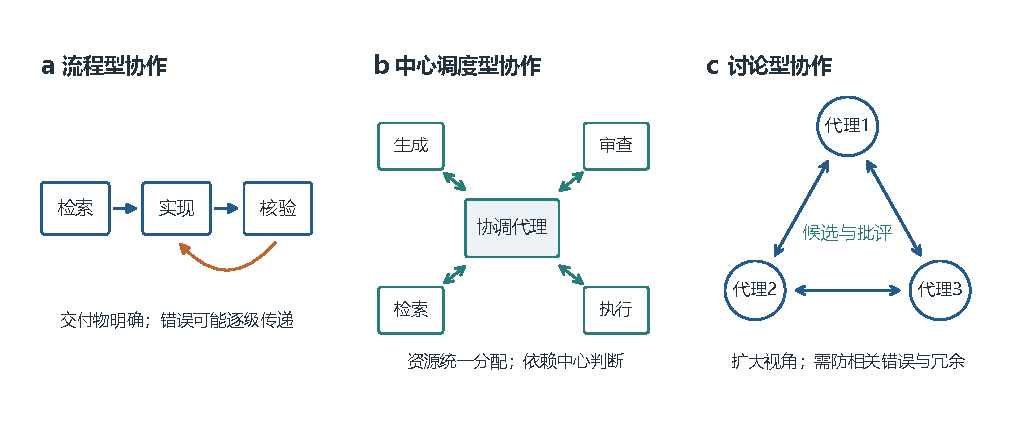
\includegraphics[width=\textwidth]{figures/review-topologies.pdf}
\caption{多智能体协作的三种基本组织形式。依据代理交互、标准化流程与多代理辩论研究归纳\cite{autogen,metagpt,debate}。
节点表示功能主体，边表示允许的交互；图示用于分析组织差异，不将某一框架限定为单一拓扑。}
\label{fig:topology}\end{figure*}

通信结构影响系统效率，也影响错误传播。
流水线可以减少无关讨论，但上游遗漏可能被下游连续接受；
中心调度便于统一判断，却形成对协调者的依赖；
自由讨论扩大了信息交换范围，也增加重复消息、状态不一致和过早形成共识的可能。
在$n$个代理每轮两两通信的理想化设置中，$T$轮对应的有向消息数为$Tn(n-1)$。
实际费用还取决于消息长度、工具调用和重试次数，但这一关系已经说明通信开销需要随协作规模一起评价。

\subsection{任务分解与标准化交付}
将研究目标拆成子任务，既是能力分配问题，也是约束传递问题。
如果任务定义只有“完成实验”或“检查结果”，后续代理仍需自行猜测哪些数据、指标和条件应被保留。
MetaGPT将标准化操作程序嵌入角色协作，使中间产物成为后续工作的共同依据\cite{metagpt}。
科研系统可以借鉴这一思路，将文献证据、实验方案、运行记录和结论依据作为不同交付对象。

标准化的作用并不是增加固定格式，而是减少信息在交接中的损失。
检索环节应说明来源支持何种判断，实验环节应保留比较条件及配置，
分析环节应区分观测结果与解释，报告环节则需要维持结论范围。
只有这些对象能够相互对应，检查者才能判断问题来自任务定义、程序实现还是结果解释。
相反，若交付仅包含经过润色的摘要，流程虽然更简洁，返工和审计却会更加困难。

任务分解还需适应研究的不确定性。
对目标明确的复现任务，固定流程通常有利于控制变量；
对假设探索任务，过早固定步骤可能限制新证据引起的方向调整。
因此，流程约束宜优先固定研究原则和交付内容，对探索路径保留一定灵活性。
这种区分能够兼顾研究过程的开放性与实验比较的可解释性。

\subsection{反馈、反思与辩论的作用条件}
ReAct将外部行动观察纳入推理过程，为科研代理调用检索和程序工具提供了基本交互模式\cite{react}。
Reflexion进一步让反馈影响后续尝试\cite{reflexion}，多代理辩论则通过交换不同回答与理由，
使系统在部分推理和事实任务中改善结果\cite{debate}。
这些工作共同说明，增加修订机会能够带来收益，但收益来源并不相同：
可能来自新证据、错误定位、候选多样性，也可能来自更多推理样本。

因此，需要区分外部反馈与语言层面的再评价。
编译器可以判断部分程序错误，测试可以检验预先规定的行为，实验仪器则提供关于物理对象的观察；
模型批评主要评价已有材料中的合理性和一致性。
它们都可能有用，但能够支持的结论范围不同。
Huang等对内在自我纠错的研究表明，没有可靠外部反馈时，所测推理任务的修订并不稳定\cite{correct}。
这与辩论方法在部分任务上的正向结果并不矛盾，因为任务、信息来源和计算设置不同。

多角色的独立性也需要具体判断。
使用相同基础模型并不必然使协作无效，但共享资料和错误前提会限制检查增量。
检索者寻找支持材料，反例搜索者专门寻找相反证据，执行者独立重算结果，
比多个角色重复评价同一段文字更容易形成互补信息。
由此可见，协作设计的重点在于构造有意义的差异，而非仅增加身份设定。

\subsection{从固定流程到搜索调度}
当研究存在多个候选方案时，协作还需要决定资源应投向哪条路径。
The AI Scientist-v2引入实验管理代理和渐进式树搜索，将候选实现、调试及改进组织为分支探索\cite{scientistv2}。
AI co-scientist则通过假设比较和演化调整候选集合\cite{cosci}。
前者的反馈更多来自可执行实验与评价，后者更侧重假设和研究建议的质量。
二者分别展示了实现空间与假设空间中的搜索控制。

搜索带来更广的探索机会，也引入候选选择偏差。
若多次尝试始终围绕测试集成绩选择方案，最终报告可能高估泛化能力；
若候选排名仅依赖同类模型判断，则可能偏好容易表述、符合常见叙事的想法。
因此，搜索效率、研究质量和评价有效性应分别报告。
对科研系统而言，保留候选淘汰原因、失败尝试和最终选择依据，
比单独展示最优分支更有助于理解其实际能力。

\section{科研应用与代表性系统}
\subsection{文献综合与研究问题形成}
文献工作既是科研智能体较易进入的场景，也是后续研究的知识基础。
PaperQA2将搜索、文献处理、证据整理与带引用的回答联系起来，并针对检索、综合及矛盾识别设计评价\cite{paperqa}。
相较于仅在给定段落上问答，这类系统需要决定继续搜索何种材料，以及何时已有证据足以回答问题。
研究中的矛盾识别结果还说明，资料综合不仅涉及归纳共识，也涉及寻找不能被同时接受的表述。
这些任务使评价从答案流畅性转向材料覆盖与来源支持，具有直接的科研实用价值。

ResearchAgent以核心论文为起点，结合学术关系和概念知识生成问题、方法与实验构想，
再通过评审代理的反馈迭代修订\cite{researchagent}。
SciAgents进一步将本体知识图谱、语言模型与多主体讨论结合，用于探索材料相关概念之间的联系\cite{sciagents}。
二者分别强调围绕论文展开的构思和图结构支持的跨概念关联。
这类方法为从已有知识中发现研究切入点提供了可操作途径，也使图组织的价值从信息检索延伸到候选生成。

不过，构思质量仍有多个层次。
新颖性关注与已有工作的差别，合理性关注机制或方法是否自洽，可检验性则要求提出可以实施的区分手段。
人工或模型评价可以检验候选是否值得进一步研究，但不能代替候选真正实施后的证据。
因此，文献与假设系统最适合被理解为研究准备和探索工具，其产出需要在实验设计阶段继续筛选。
这一定位能够保留系统的创造性价值，也避免把构思评分直接解释为发现成功。

\subsection{计算实验与端到端研究}
计算科研具有数据、程序和指标可被统一工具链处理的特点，是端到端研究的重要试验场。
The AI Scientist早期系统将创意生成、代码修改、运行、分析、写作与模拟评审连接起来\cite{scientist}。
其预设模板限定了初始研究空间，但也降低了环境配置与基础实现的不确定性，便于集中考察想法生成和实验迭代。
第二版系统减少对人工代码模板的依赖，使用实验树搜索扩展候选，并引入视觉语言反馈改善图表与呈现\cite{scientistv2}。
从固定模板到搜索式实验管理，反映了自动科研由局部修改向更开放实现空间的发展。

2026年的期刊报告同时研究聚焦模式与开放模式，并进一步讨论自动评审及实际工作坊评审\cite{scientistjournal}。
这比仅由系统内部评价生成论文提供了更多外部参照。
但工作坊个案的评价范围、主题设置和接受条件仍需与通常意义上的广泛科学贡献区分。
早期系统、第二版与期刊报告属于同一研究脉络，不能作为三次独立的全面能力验证累加。

Agent Laboratory采用不同的协作定位：从人提供的研究想法出发，组织文献、实验与报告，
并允许在各阶段引入人的反馈\cite{lab}。
其价值在于把自动化目标与研究者的已有目标相结合，而不要求系统独立决定所有问题。
原文同时比较模型后端、人工评价和不同参与方式，报告了特定设置中自动总体评分6.1/10与人工3.8/10的差异。
这一结果表明，研究报告的可读性、实验质量和评审模型偏好需要分开评价。
对于协作式工具，实际帮助可能体现为降低实现负担，也可能体现为研究者更容易发现计划中的问题，
因而仅用最终论文评分还不能完整衡量其效用。

\subsection{假设搜索与跨学科研究协作}
AI co-scientist围绕专家给定的目标，组织生成、反思、排序、演化等功能代理，
通过候选比较与迭代形成研究建议\cite{cosci}。
这种设计将计算资源用于扩大和修订假设空间，与按既定方案执行一次实验不同。
其排序反馈有助于筛选候选，但排名反映的是比较标准下的相对优势，不能直接解释为命题成立的概率。

该研究在药物再利用、肝纤维化靶点及细菌基因转移机制等方向报告验证案例\cite{cosci}。
各案例的证据性质不同：细胞或类器官结果提供特定实验体系中的支持，
与尚未公开的实验机制相符合，则体现另一种知识推断能力。
这些案例说明候选生成可以与真实科研检验衔接，但其一般化范围仍取决于问题选择和后续实验。

Virtual Lab以负责人代理和专业代理组成研究会议，由人类提供高层反馈，
将蛋白质语言模型、结构预测和分子能量评价整合到纳米抗体设计流程\cite{virtual}。
论文选择92个候选进行实验表征，既呈现了有前景的候选，也显示计算指标与实际功能的差异。
其中78个候选具有更高的相应结构置信度指标，60个具有更优的Rosetta结合能，
但不同亲本系列的实际结合表现并不一致。
这说明专用计算模型、代理组织和实验验证承担不同作用，不能仅凭代理参与就把所有收益归为LLM推理。
对跨学科研究而言，多代理更有意义的贡献是组织已有专长和工具，并使不同研究环节形成可追踪联系。

\subsection{专业工具与实体实验}
ChemCrow将18种专业工具与语言模型结合，用于化学相关问题、合成规划及实验任务\cite{chemcrow}。
专门工具补充了基础模型难以可靠完成的化学计算、检索和执行能力。
这一设计体现了通用代理与领域工具之间的分工：模型负责解释目标和选择步骤，工具负责具有明确输入输出的专业操作。
工具覆盖范围、输入表达和输出解释因而与模型能力同样重要。

Coscientist进一步将网络检索、装置文档、代码执行和实验设备整合，展示化学实验从自然语言要求到执行与产物检查的过程\cite{chem}。
图\ref{fig:physical}左侧概括其关键步骤，右侧保留原论文的实验谱图。
在这一流程中，装置文档能够帮助修正调用方式，色谱与质谱则提供区别于语言评价的产物证据。
研究因此不只依赖系统是否声称完成任务，还可以检查实验输出与参照物之间的关系。

\begin{figure*}[t]\centering
\begin{minipage}[c]{.49\textwidth}\centering
\begin{tikzpicture}[node distance=4mm,b/.style={draw=ZJUIBlue,rounded corners=1.5pt,text width=62mm,minimum height=9mm,align=center,font=\small},a/.style={-{Stealth[length=2mm]},thick,draw=ZJUIBlue}]
\node[font=\bfseries\small] (title) {从任务指令到可检查的实验输出};
\node[b,below=3mm of title] (r) {查阅文献与装置文档};
\node[b,below=of r] (p) {选择方案并生成执行程序};
\node[b,below=of p] (e) {调用液体处理与分析设备};
\node[b,below=of e] (v) {将产物测量与参照数据比较};
\draw[a](r)--(p);\draw[a](p)--(e);\draw[a](e)--(v);
\draw[a,draw=EvidenceGreen](e.east) to[out=0,in=0] (p.east);
\node[below=3mm of v,font=\footnotesize,align=center,text width=66mm] {装置反馈修正操作；测量结果支持实验判断。};
\end{tikzpicture}
\end{minipage}\hfill
\begin{minipage}[c]{.235\textwidth}\centering
{\small Suzuki反应}\par\vspace{2mm}
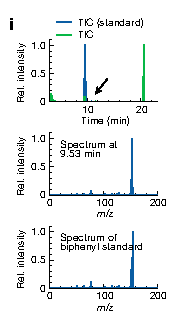
\includegraphics[width=\linewidth]{figures/coscientist-suzuki.pdf}
\end{minipage}\hfill
\begin{minipage}[c]{.235\textwidth}\centering
{\small Sonogashira反应}\par\vspace{2mm}
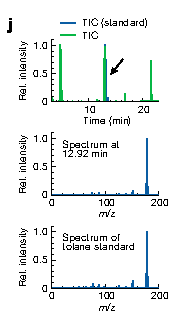
\includegraphics[width=\linewidth]{figures/coscientist-sonogashira.pdf}
\end{minipage}
\caption{科研代理与实体实验验证的衔接。左部依据Coscientist流程归纳\cite{chem}；
右部摘自Boiko等原图5i、5j，分别包含色谱及对应质谱与标准参照。图中曲线、坐标与数值保持原样，仅提取面板并调整排列。
原图版权为作者，依据\href{https://creativecommons.org/licenses/by/4.0/}{CC BY 4.0}转载；数据不是本文实验结果。}
\label{fig:physical}\end{figure*}

实体反馈提高了某些判断的可检查性，也使资源与操作约束更加突出。
Coscientist的部分物理操作仍由人工完成，可探索的试剂和设备范围也由实验设置限定\cite{chem}。
因此，系统应在明确资源边界内评价，不宜把特定装置上的成功直接扩展为开放实验室中的普遍自主能力。
与纯计算场景相比，实体系统更需要在计划阶段考虑操作权限、异常中止、测量噪声和验证成本。

\subsection{不同科研路径的比较}
表\ref{tab:systems}从研究对象与反馈方式总结代表系统。
文献与构思系统的主要产物是证据综合和候选问题，计算系统便于反复执行，实体系统则可以获得更直接的经验观察。
不同路线的自动化覆盖与验证深度相互独立：覆盖更多阶段可以减少人工交接，但也增加错误跨阶段传播的机会；
加入实验测量能够检验具体命题，却仍然依赖有效的对照与解释。
因此，更有意义的比较不是给系统排列统一自主等级，而是说明它们在哪些条件下推进了哪些研究活动。

\begin{table*}[t]\centering\tabletext
\caption{代表性科研系统的主要组织方式与证据来源。不同报告之间的任务、模型、工具和人工参与不同，不作统一成绩比较。}
\label{tab:systems}
\begin{tabularx}{\textwidth}{@{}>{\raggedright\arraybackslash}p{29mm}YYY@{}}\toprule
系统 & 研究对象与组织重点 & 反馈或验证方式 & 主要解释边界\\\midrule
PaperQA2\cite{paperqa} & 文献检索、综合与矛盾识别 & 文献任务基准及专家比较 & 文献综合能力不等同于实验发现能力\\
ResearchAgent / SciAgents\cite{researchagent,sciagents} & 论文关系、概念图谱与迭代构思 & 评审反馈、人工或模型评价与案例 & 候选质量仍需后续实施和检验\\
The AI Scientist系列\cite{scientist,scientistv2,scientistjournal} & 模板研究、实验搜索与论文生成 & 程序实验、自动评审及工作坊案例 & 同一研究系列；个案评审有其适用范围\\
Agent Laboratory\cite{lab} & 人给定想法上的研究协作 & 人工评价、后端与参与方式比较 & 人工帮助及评价差异需单独报告\\
AI co-scientist\cite{cosci} & 多候选生成、比较和演化 & 专家反馈与部分生物医学实验 & 排序不是命题真值，验证类型存在差异\\
Virtual Lab\cite{virtual} & 跨学科会议与专用计算工具整合 & 纳米抗体设计后的实验表征 & 计算指标、表达与功能为不同评价目标\\
ChemCrow / Coscientist\cite{chemcrow,chem} & 专业工具调用与实体执行 & 专家检查、仪器观察及产物分析 & 工具覆盖、装置条件和人工操作限制范围\\\bottomrule
\end{tabularx}\end{table*}

\section{实证评价}
\subsection{评价对象}
科研系统可以交付答案、程序、实验方案或一篇论文，评价不能只依据同一个文本分数。
文献回答需要检查来源支持，程序任务需要核对执行结果，开放研究还涉及选题、对照和解释。
表\ref{tab:benchmarks}列出几种常用评价工作的对象；它们回答不同问题，并没有形成一个统一的科研能力量尺。

ScienceAgentBench从44篇同行评审论文中提取102项数据驱动任务，要求系统生成独立程序并保存输出\cite{sciencebench}。
有效执行率（valid execution rate，VER）检查能否执行并产生规定输出；任务成功率（success rate，SR）进一步检查是否达到各项任务的标准。
这一差别使实验中一个常被忽略的事实可见：程序已经运行，任务仍可能没有完成。
基准针对的是研究工作流中的具体计算任务，而非一项完整发现。

RE-Bench采用7个开放机器学习研究工程环境，并引入人类专家尝试\cite{rebench}。
其人与代理的相对表现随时间预算改变：代理在短预算下表现较强，而人类在更长预算下取得更明显的后续收益。
这一结果提醒研究者，“超过专家”必须与任务、时间和尝试分配一起报告。
代理快速搜索若干方案与专家长期改进同一研究，并不是可以不计资源直接比较的活动。

\begin{table*}[t]\centering\tabletext
\caption{科研评价工作的任务及测量内容。}
\label{tab:benchmarks}
\begin{tabularx}{\textwidth}{@{}L{39mm}L{48mm}Y@{}}\toprule
\textbf{评价工作} & \textbf{任务材料} & \textbf{主要测量内容}\\\midrule
\tabname{PaperQA2 / LitQA2}{paperqa} & 检索、综合与矛盾识别 & 回答质量、来源支持及专家比较\\[5pt]
\tabname{ScienceAgentBench}{sciencebench} & 44篇论文中的102项任务 & VER、SR、代码相似度及费用\\[5pt]
\tabname{RE-Bench}{rebench} & 7个研究工程环境 & 不同时间预算下的任务收益\\[5pt]
\tabname{MAST}{mast} & 多代理轨迹及失败案例 & 规范、协调和核验环节的失败类型\\[5pt]
科研过程审计\cite{pitfalls} & 100个受控审计案例 & 方法学缺陷识别准确率\\\bottomrule
\end{tabularx}
\tabnote{注：VER为有效执行率，SR为任务成功率。各工作的任务、预算及评分定义不同，成绩不可直接合并。}
\end{table*}

\subsection{执行反馈的实证表现}
图\ref{fig:sciencebench}重绘ScienceAgentBench中两个模型在三种框架下的结果。
直接生成（Direct）提供简单参照，Self-Debug允许依据执行反馈修订，OpenHands CodeAct提供更广的交互动作。
原协议对每项任务独立运行三次，依次按SR、VER、CodeBERTScore和较低费用择优，再汇总入选运行。
这些数值因此反映择优后的表现，不是一次运行的均值。

在无专家知识的设置中，Claude 3.5 Sonnet与Self-Debug结合的VER为92.2\%，SR却为32.4\%；GPT-4o对应为83.3\%与22.6\%\cite{sciencebench}。
两者分别相差59.8和60.7个百分点。
仅有汇总数据还不能把差距归因到某一种错误，却足以否定“程序能运行就完成了任务”的判断。
执行反馈能排除一部分实现问题，数据处理和科学目标仍需要单独检查。

资源投入也没有与成功率形成简单的单调关系。
Claude 3.5 Sonnet使用OpenHands时，平均API费用为0.958美元、SR为21.6\%；Self-Debug对应为0.057美元和32.4\%\cite{sciencebench}。
这里比较的是相同模型、相同基准下的框架配置，说明更大的动作空间不一定更容易被有效利用。
它支持将简单反馈方案列为基线，尚不能推广成某一框架在所有任务中更优。
同样，这组实验比较的是代理框架，并未直接分离多代理角色协作的效果。

\begin{figure*}[t]\centering
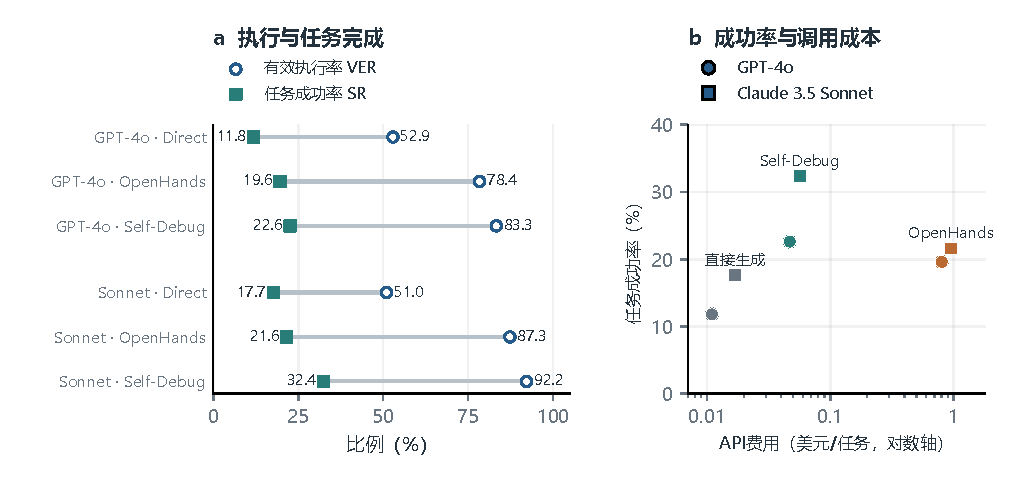
\includegraphics[width=\textwidth]{figures/review-sciencebench.pdf}
\caption{ScienceAgentBench中六组配置的执行、成功与费用。数据取自文献\cite{sciencebench}表3（v3，PDF第8页），均不提供专家知识，共102项任务，每项三次独立运行后择优。
(a) VER与SR；(b) SR与平均API调用费用，对数横轴。模型和美元费用对应原报告时期；点表示表3汇总结果，不是三次运行均值。}
\label{fig:sciencebench}\end{figure*}

\subsection{科研过程审计}
MAST将多代理失败整理为规范与系统设计、主体间失配以及任务核验等类别\cite{mast}。
这类过程分类有助于定位问题：目标理解错误、交接丢失条件和过早结束任务，可能需要完全不同的修正。
只看最终论文，往往无法区分这些原因。

Luo等进一步考察自动科研中的基准选择偏差、数据泄漏、指标误用、事后选择和数据替换或编造等缺陷\cite{pitfalls}。
在其100个正负均衡案例上，审计模型仅阅读论文时总体准确率为55\%，同时获得日志和代码后提高到82\%。
图\ref{fig:audit}以各类识别正确的案例数展示这一变化。
数据泄漏从11/20提高到18/20，事后选择从10/20提高到14/20，说明过程材料的帮助在不同问题上也有差异。

\begin{figure*}[t]\centering
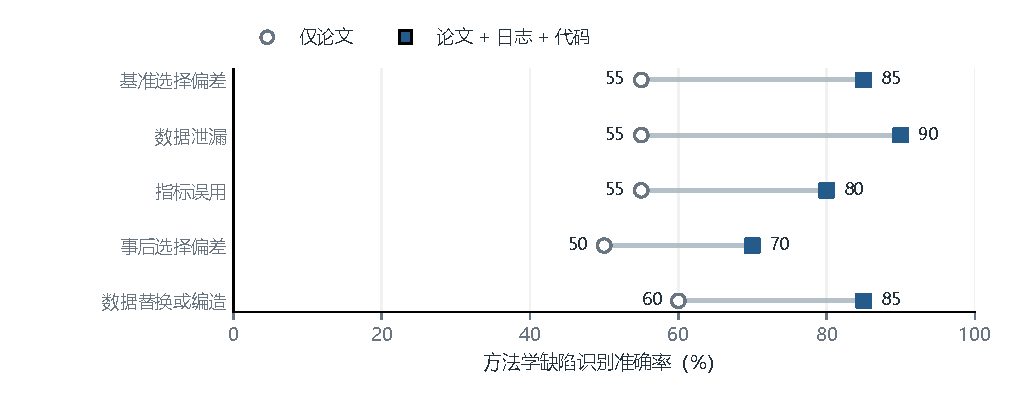
\includegraphics[width=\textwidth]{figures/review-audit.pdf}
\caption{补充过程材料后的缺陷识别。由文献\cite{pitfalls}第6.2节及表11（v2，PDF第16--18页）中的准确率换算为正确案例数；每类20例，阳性、阴性各10例，部分缺陷为原作者受控注入。
审计模型为gemini-2.5-flash-preview-05-20；日志与代码同时加入，未分别估计二者贡献。}
\label{fig:audit}\end{figure*}

这一实验支持提供过程材料，却没有测量真实科研中缺陷有多常见。
案例数量、受控注入和正负比例规定了结果的解释范围；图中也不据此补出总体发生率或不确定区间。
更值得注意的是，论文与过程记录能够回答的问题不同。
前者陈述最终采用的分析，后者可能揭示筛掉了哪些尝试、何时查看过测试结果、训练和测试数据究竟如何使用。
自动化越深入，这种差别越有可能影响对研究的判断。

\subsection{协作增益的归因分析}
若要识别协作贡献，单代理基线应具有相应的检索、执行和重试机会，并尽量匹配模型、工具、预算与人工帮助。
否则，多代理系统获得的提升虽是系统层面的真实差异，却未必来自角色分工。
消融还需要说明资源如何重新分配：删除检查者并同时减少调用次数，不能单独回答检查角色是否必要。

更有针对性的比较是保留总预算后合并角色，或保留角色数量但改变检查者能访问的材料。
前者观察分工与通信是否值得，后者观察检查的信息来源是否产生增益。
对长期任务，还可检查系统在一项关键判断被推翻后，能否找出受影响的后续实验。
这些评价比单独增加一个最终答案分数更难，但也更贴近科研协作实际要解决的问题。

\section{综合讨论与研究展望}
\subsection{由流程自动化转向研究有效性}
前述研究表明，知识增强、长期记忆与多代理协作分别处理不同瓶颈，系统能力来自其配合，而不是某个机制名称。
更强检索可以改善问题所依据的材料，长期记忆可以减少反复重建上下文，协作则可以组织专业工具与检查过程。
这些进展确实扩大了自动科研的任务范围。
然而，跨阶段组合也使局部错误更容易影响后续选择，因此评价对象应从单步回答继续扩展到研究依赖关系。

本文认为，科研系统值得长期保留的基本对象，应是具有明确依据和适用范围的研究判断。
每项关键判断关联其来源、实验条件和反证，后续任务才能知道哪些内容可以继续采用、哪些仍需验证。
当数据处理被修正时，系统应识别受影响的结果与结论，而不是只重新生成一篇措辞一致的报告。
这一要求将知识图谱的关联能力、记忆的版本维护和协作的返工控制联系起来，也为长期科研评价提供了更具体的观察对象。

\subsection{知识组织与研究记忆的互补关系}
课堂中关于图式知识组织和自主记忆的讨论，反映了两种不同需求。
图结构适合相对稳定的概念关联和跨文献主题，任务记忆则需要快速容纳尚不确定的尝试、解释与异常。
若全部内容都按稳定知识处理，新假设可能过早固化；若只保留自由对话，重要关系又难以持续利用。
因此，二者结合的关键不是采用相同存储格式，而是明确什么信息在何种条件下可以转入较稳定的知识状态。

一个可行方向是保留观察、解释和结论之间的依赖，让反证能够改变状态而不抹去历史。
常规记录可以压缩，影响研究方向的判断则保留更完整依据。
图\ref{fig:cycle}给出了本文的综合理解：检索和候选生成扩展探索范围，区分性实验提供新观察，
记忆更新再影响下一轮选择。
这一路径同时强调信息获取与认识修订，能够避免把已有判断在知识库和代理之间反复传递当成新的支持。

\begin{figure*}[t]\centering
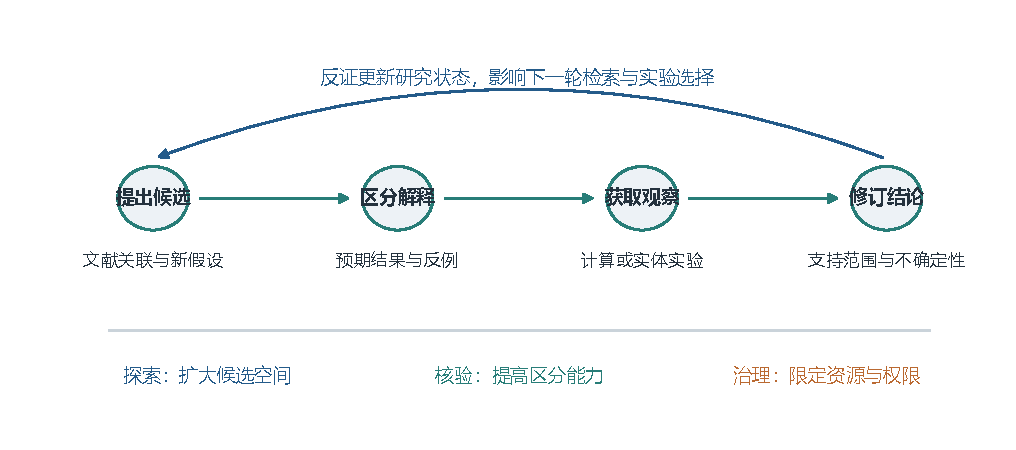
\includegraphics[width=\textwidth]{figures/review-evidence-cycle.pdf}
\caption{基于综述形成的研究闭环理解。候选生成、区分解释、外部观察与结论修订相互联系，
探索、核验和资源治理分别提供不同约束。该图为本文讨论框架，未声称已经实现或经新实验验证。}
\label{fig:cycle}\end{figure*}

\subsection{探索效率与验证成本的共同约束}
候选生成速度提高之后，系统瓶颈可能从提出想法转移到判断哪些想法值得继续研究。
更多代理能够产生更多方案，却未必增加实验资源或领域审查能力。
因此，研究预算需要同时覆盖探索与核验，并考虑不同候选能否被现有数据或低成本实验有效区分。
对于验证代价较高的问题，单纯增加候选数可能增加筛选负担，而不是提高科研效率。

验证也不应被简化为与已有共识的一致程度。
新假设往往超出现有结论，审查的作用是确认事实基础、逻辑关系与可检验条件，而非要求所有推测都已被证明。
允许系统明确保留“尚待检验”的判断，能够在探索空间与科学审慎之间形成更合理的平衡。
相应地，评价应分别报告新颖性、可行性和证据支持度，不宜由一个语言偏好分数替代。

\subsection{协作规模与人工参与的任务适配}
科研多代理更适合任务依赖复杂、工具异质且交付可检查的场景。
对于局部事实检索，增加角色可能主要增加通信成本；对跨学科设计，不同功能主体与专用工具之间的配合则更有价值。
因此，协作规模宜由任务结构和实际消融决定。
未来系统可以根据当前不确定性调整参与角色，而非从开始到结束维持固定人数和相同讨论模式。

人的作用也需要从简单的“是否介入”进一步细化。
问题选择、对照设计、异常解释和结论范围通常具有较高判断价值；常规检索、运行和材料整理则更适合交由工具处理。
在前者设置清晰检查点，有助于把有限专家时间用于最影响研究有效性的环节。
同时，评价需要记录人工输入与修改程度，才能判断系统是在替代劳动、放大已有能力，还是把工作转移到了未被计量的审查过程。

\begin{table*}[t]\centering\tabletext
\caption{由本文分析形成的可检验研究议题。以下为研究设计建议，未报告本项目新实验。}
\label{tab:agenda}
\begin{tabularx}{\textwidth}{@{}>{\raggedright\arraybackslash}p{32mm}YY@{}}\toprule
研究议题 & 可采用的对照设计 & 需要观察的结果\\\midrule
来源与状态管理的贡献 & 相同工具和预算下，比较无类型记忆与来源、状态可区分的记忆 & 错误重复、反证利用、关键判断可重建程度\\
协作结构的必要性 & 保留调用预算和权限，比较单代理、固定分工及动态调度 & 完成质量、通信开销、中断与返工分布\\
独立检查的有效性 & 保留角色数，改变检查者能访问的原文、数据与执行记录 & 缺陷识别、误报、修正成功和检查成本\\
人机协作的价值位置 & 记录并比较目标、实验设计及结果解释阶段的人工介入 & 质量改善、专家时间、修改量及研究者负担\\\bottomrule
\end{tabularx}\end{table*}

\subsection{长期评价与本文局限}
真实科研往往没有立即可知的唯一答案，目标也可能随新证据改变。
短任务基准适合比较局部能力，但对长期研究中的错误恢复、方向调整和失败价值覆盖不足。
未来评价应保留跨阶段轨迹，并在可行时加入独立执行者、预先保留任务及后续复查，
考察系统能否在新证据下更新既有结论，而不只是完成一次既定流程。

本文以知识、记忆和协作为主要分析线索，没有完整覆盖训练式多代理优化、基础模型训练和所有学科应用。
所引系统的模型、任务、工具与人工参与不同，本文不进行跨论文效应合并。
重绘数据图仅呈现原论文内部比较，转载谱图保留原始实验属性，均未作为本项目新结果。
此外，早期模型上的数值表现不代表当前系统水平；其揭示的评价问题需要在新模型和新任务中继续检验。

\section{结语}
大语言模型驱动的科研多智能体系统，正在将知识获取、工具执行和研究交流整合到持续工作流中。
检索增强改善外部知识的访问，层次与图组织支持跨材料综合，反思和分层记忆延续任务经历，
协作协议与搜索调度则组织多个主体在研究过程中的配合。
代表系统展示了从文献综合到计算实验、再到实体测量的多种路径，也说明不同科研活动需要不同形式的反馈与验证。

综合现有证据，协作规模、自动化覆盖和科研可信度应分别描述。
可靠系统需要保留来源、实验条件、失败尝试及修订依据。
知识与研究状态的协同维护、探索和验证资源的联合分配，以及关键节点的人机协作，
是值得持续研究的方向。
科研智能体的价值，最终应体现为更有效、更可复查的研究过程与产出。

% BODY-END
\FloatBarrier
\begingroup\fontsize{9.5}{13.2}\selectfont\raggedright
\interlinepenalty=10000
\begin{thebibliography}{99}
\bibitem{rag} Lewis P, Perez E, Piktus A, et al. Retrieval-Augmented Generation for Knowledge-Intensive NLP Tasks[EB/OL]. 2020. arXiv:2005.11401v4. \url{https://arxiv.org/abs/2005.11401v4}.
\bibitem{react} Yao S, Zhao J, Yu D, et al. ReAct: Synergizing Reasoning and Acting in Language Models[EB/OL]. 2022. arXiv:2210.03629v3. \url{https://arxiv.org/abs/2210.03629v3}.
\bibitem{autogen} Wu Q, Bansal G, Zhang J, et al. AutoGen: Enabling Next-Gen LLM Applications via Multi-Agent Conversation[EB/OL]. 2023. arXiv:2308.08155v2. \url{https://arxiv.org/abs/2308.08155v2}.
\bibitem{scientist} Lu C, Lu C, Lange R T, et al. The AI Scientist: Towards Fully Automated Open-Ended Scientific Discovery[EB/OL]. 2024. arXiv:2408.06292v3. \url{https://arxiv.org/abs/2408.06292v3}.
\bibitem{lab} Schmidgall S, Su Y, Wang Z, et al. Agent Laboratory: Using LLM Agents as Research Assistants[EB/OL]. 2025. arXiv:2501.04227v2. \url{https://arxiv.org/abs/2501.04227v2}.
\bibitem{memgpt} Packer C, Wooders S, Lin K, et al. MemGPT: Towards LLMs as Operating Systems[EB/OL]. 2023. arXiv:2310.08560v2. \url{https://arxiv.org/abs/2310.08560v2}.
\bibitem{graphrag} Edge D, Trinh H, Cheng N, et al. From Local to Global: A Graph RAG Approach to Query-Focused Summarization[EB/OL]. 2024. arXiv:2404.16130v2. \url{https://arxiv.org/abs/2404.16130v2}.
\bibitem{middle} Liu N F, Lin K, Hewitt J, et al. Lost in the Middle: How Language Models Use Long Contexts[EB/OL]. 2023. arXiv:2307.03172v3. \url{https://arxiv.org/abs/2307.03172v3}.
\bibitem{generative} Park J S, O'Brien J C, Cai C J, et al. Generative Agents: Interactive Simulacra of Human Behavior[EB/OL]. 2023. arXiv:2304.03442v2. \url{https://arxiv.org/abs/2304.03442v2}.
\bibitem{correct} Huang J, Chen X, Mishra S, et al. Large Language Models Cannot Self-Correct Reasoning Yet[EB/OL]. 2023. arXiv:2310.01798v2. \url{https://arxiv.org/abs/2310.01798v2}.
\bibitem{cosci} Gottweis J, Weng W H, Daryin A, et al. Towards an AI co-scientist[EB/OL]. 2025. arXiv:2502.18864v1. \url{https://arxiv.org/abs/2502.18864v1}.
\bibitem{virtual} Swanson K, Wu W, Bulaong N L, et al. The Virtual Lab of AI agents designs new SARS-CoV-2 nanobodies[J]. Nature, 2025, 646: 716--723. \url{https://doi.org/10.1038/s41586-025-09442-9}.
\bibitem{chem} Boiko D A, MacKnight R, Kline B, et al. Autonomous chemical research with large language models[J]. Nature, 2023, 624: 570--578. \url{https://doi.org/10.1038/s41586-023-06792-0}.
\bibitem{mast} Cemri M, Pan M Z, Yang S, et al. Why Do Multi-Agent LLM Systems Fail?[EB/OL]. 2025. arXiv:2503.13657v2. \url{https://arxiv.org/abs/2503.13657v2}.
\bibitem{pitfalls} Luo Z, Kasirzadeh A, Shah N B. The More You Automate, the Less You See: Hidden Pitfalls of AI Scientist Systems[EB/OL]. 2025. arXiv:2509.08713v2. \url{https://arxiv.org/abs/2509.08713v2}.
\bibitem{skills} Kassis T, Agarwal V, He Y, et al. Scientific Agent Skills: A Library of Procedural Knowledge for Research Agents[EB/OL]. 2026. \url{https://doi.org/10.48550/arXiv.2609.00065}.
\end{thebibliography}
\vspace{3mm}\noindent\textbf{资料与工具说明}\quad
本文为叙述性综述，未重新运行所引系统的实验。
资料整理、文字修订与图表代码由Codex辅助完成，参考Scientific Agent Skills的综述和可视化工作流\cite{skills}；
该文献仅记录工具来源，不计入15项研究的比较。
数值图由公开表格重绘，概念图为本文归纳。当前为供作者核阅的课程修订稿。
\endgroup

\end{document}
